\chapter{Arsitektur dan Teknologi Sistem}

\section{Arsitektur Sistem}

\begin{figure}[H]
    \centering
    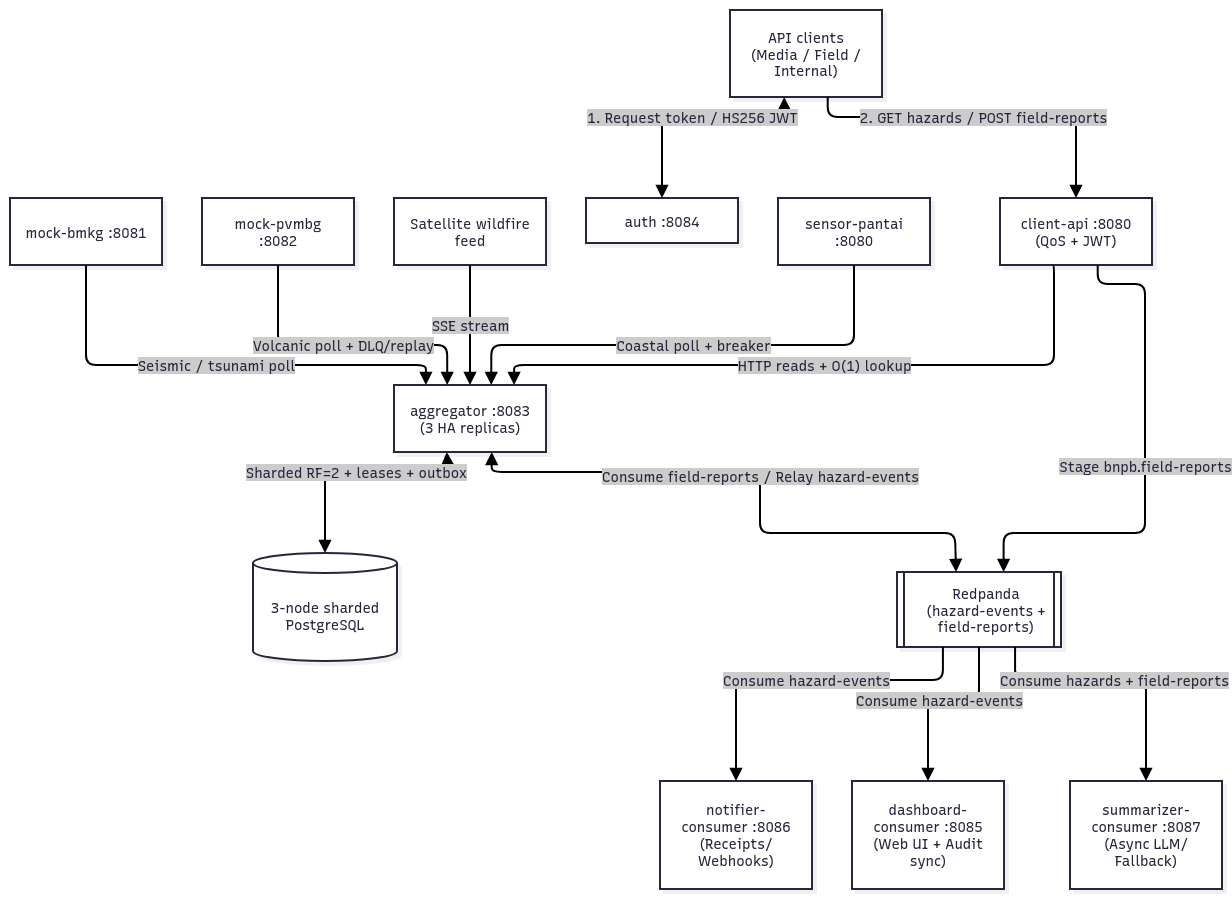
\includegraphics[width=0.95\textwidth]{figures/arsitektur-m2.png}
    \caption{Arsitektur Sistem Terdistribusi Platform Koordinasi Kebencanaan BNPB Milestone~2.}
    \label{fig:arsitektur_m2}
\end{figure}

Platform Koordinasi Kebencanaan BNPB pada Milestone~2 menerapkan arsitektur \textit{event-driven microservices} multi-node di atas kluster Kubernetes (k3s) beranggotakan tiga node berkernel Linux terpisah (\texttt{aqua}, \texttt{ruby}, dan \texttt{akane}), serta dilengkapi simulasi lokal berbasis Docker Compose. Sistem tersusun atas delapan modul Go independen bersama komponen penyimpanan terpartisi, \textit{message broker}, dan tumpukan observabilitas yang terbagi ke dalam empat lapisan utama (Gambar~\ref{fig:arsitektur_m2}):

\begin{enumerate}
    \item \textbf{Lapisan Sumber Data Hulu:} Mencakup lima sumber data bencana, yakni \texttt{mock-bmkg} (gempa bumi dan tsunami), \texttt{mock-pvmbg} (aktivitas gunung api beserta simulasi gangguan dan evolusi skema), \texttt{sensor-pantai} (pelampung pesisir), aliran SSE satelit kebakaran eksternal, serta laporan lapangan petugas melalui \texttt{client-api}.
    \item \textbf{Lapisan Inti Koordinasi, Penyimpanan, dan Bus Event:} Terdiri atas \texttt{aggregator} (\textit{High Availability} multi-replika), tiga unit StatefulSet PostgreSQL~16 terpartisi (\texttt{store-aqua}, \texttt{store-ruby}, dan \texttt{store-akane}) dengan tiga shard logis dan replikasi lintas node ($RF=2$), serta \textit{message broker} Redpanda untuk topik \texttt{bnpb.hazard-events} dan \texttt{bnpb.field-reports}.
    \item \textbf{Lapisan Akses Publik dan Konsumen Hilir:} Lalu lintas eksternal dirutekan melalui Traefik Ingress menuju \texttt{auth} dan \texttt{client-api} (dengan \textit{autoscaling} HPA), sedangkan sisi hilir asinkron diisi oleh tiga konsumen independen: \texttt{dashboard-consumer}, \texttt{notifier-consumer}, dan \texttt{summarizer-consumer} yang terintegrasi dengan LLM lokal (\texttt{qwen3.5:9b}).
    \item \textbf{Lapisan Observabilitas Terpadu:} Terdiri atas Prometheus untuk pengumpulan metrik layanan, Grafana Tempo untuk penyimpanan \textit{distributed tracing}, serta Grafana untuk visualisasi dasbor pemantauan dan penelusuran latensi.
\end{enumerate}

\section{Tanggung Jawab Setiap Service}
Setiap komponen memiliki batas tanggung jawab yang terdefinisi tegas sebagai berikut.

\begin{itemize}
    \item \textbf{\texttt{mock-bmkg}:} Menyimulasikan data gempa bumi dan peringatan tsunami berkorelasi dengan autentikasi \textit{API key}, latensi rendah, serta pembangkitan data berkala.
    \item \textbf{\texttt{mock-pvmbg}:} Menyimulasikan laporan aktivitas gunung api berautentikasi \textit{Bearer token}, dilengkapi rute administratif untuk menyimulasikan pemadaman layanan dan evolusi skema data.
    \item \textbf{\texttt{sensor-pantai}:} Kontainer \textit{black-box} simulasi pelampung pantai (\texttt{COASTAL}) berautentikasi \textit{Bearer token} dengan data fluktuatif dan potensi data usang (\textit{stale}) untuk menguji ketahanan jalur ingesti.
    \item \textbf{\texttt{aggregator}:} Koordinator inti ingesti dan pemilik tunggal penyimpanan kanonis terpartisi ($RF=2$). Tanggung jawab utamanya mencakup empat hal:
    \begin{itemize}
        \item \textbf{Koordinasi sumber:} menjaga eksklusivitas ingesti per sumber melalui \textit{leader lease} dan \textit{monotonic fencing token}.
        \item \textbf{Ingesti multisumber dan ketahanan:} menarik data BMKG, PVMBG (beserta karantina DLQ dan \textit{replay} otomatis), serta \texttt{sensor-pantai} (dengan \textit{circuit breaker}, \textit{fallback cache}, dan karantina); menyimak aliran SSE satelit kebakaran; serta memproses laporan lapangan dari Redpanda.
        \item \textbf{Normalisasi dan persistensi:} menormalisasi seluruh data ke model kanonis \texttt{HazardEvent}, menyimpannya secara tereplikasi pada 3 shard PostgreSQL, lalu menerbitkannya ke \texttt{bnpb.hazard-events} melalui \textit{Transactional Outbox Relay}~\cite{richardson2018microservices}.
        \item \textbf{Antarmuka internal:} menyediakan Internal API pencarian bahaya, titik pemeriksaan status karantina/\textit{fallback}, serta Internal Audit API untuk rekonsiliasi data.
    \end{itemize}
    \item \textbf{\texttt{auth}:} Mengelola kredensial klien (\texttt{media}, \texttt{field}, \texttt{internal}), menerbitkan token akses JWT ber-\textit{scope}~\cite{rfc7519}, serta menangani rotasi \textit{refresh token} dengan deteksi penggunaan ulang (\textit{replay revocation}).
    \item \textbf{\texttt{client-api}:} Gerbang HTTP publik yang memvalidasi JWT secara lokal, membatasi proyeksi atribut sesuai \textit{scope}, menerapkan \textit{Priority QoS Load Shedding} untuk melindungi lalu lintas petugas lapangan, meneruskan pencarian bahaya ke \texttt{aggregator}, serta melakukan \textit{durable staging} laporan lapangan (\texttt{POST /api/v1/field-reports}) secara idempoten ke Redpanda.
    \item \textbf{\texttt{dashboard-consumer}:} Menyajikan antarmuka dasbor analitik web dan API JSON dari proyeksi \textit{event} Kafka yang diselaraskan berkala dengan Audit API, lengkap dengan penanda \texttt{PARTIAL DATA} saat sebagian shard tidak terjangkau.
    \item \textbf{\texttt{notifier-consumer}:} Mengevaluasi ambang peringatan darurat lintas jenis bahaya, melakukan deduplikasi notifikasi berbasis sidik jari \textit{payload}, mencatat tanda terima log, dan meneruskan \textit{webhook} opsional.
    \item \textbf{\texttt{summarizer-consumer}:} Menyusun ringkasan situasional multi-bencana secara \textit{non-blocking} menggunakan LLM lokal (\texttt{qwen3.5:9b}) dengan mekanisme \textit{extractive fallback} deterministik dan pelabelan hasil generatif yang eksplisit.
    \item \textbf{\texttt{prometheus}, \texttt{tempo}, \texttt{grafana}:} Mengumpulkan metrik seluruh replika layanan, menyimpan jejak \textit{distributed tracing} OTLP, serta menampilkan dasbor pemantauan terpadu.
\end{itemize}

\section{Protokol Komunikasi Antarservice}
Komunikasi antarservice dalam sistem dipisahkan berdasarkan kebutuhan sinkronisasi, aliran data kontinu, reliabilitas pengiriman event, serta observabilitas:

\begin{itemize}
    \item \textbf{Komunikasi Sinkron (HTTP/1.1 REST + JSON):} Digunakan pada jalur akses publik maupun internal yang bersifat \textit{request--response}. Klien eksternal mengakses \texttt{auth}, \texttt{client-api}, \texttt{dashboard-consumer}, \texttt{summarizer-consumer}, \texttt{grafana}, serta Audit API (\texttt{audit-aat.darsu.dev}) melalui Traefik Ingress. Secara internal, \texttt{client-api} memanggil \texttt{aggregator:8083} (batas waktu 5 detik per permintaan), \texttt{dashboard-consumer} melakukan sinkronisasi ke Audit API dengan \texttt{AUDIT\_TOKEN}, \texttt{aggregator} menarik data dari \texttt{mock-bmkg}, \texttt{mock-pvmbg}, dan \texttt{sensor-pantai}, sedangkan \texttt{summarizer-consumer} mengirim permintaan inferensi berprotokol OpenAI-compatible ke \texttt{llama-server} (\texttt{10.5.24.125:11434}). Seluruh jalur HTTP mempropagasi \texttt{X-Correlation-ID} dan konteks pelacakan W3C \texttt{traceparent}.
    \item \textbf{Komunikasi \textit{Server-Sent Events} / SSE over HTTPS:} Pemegang \textit{lease} \texttt{source:SATELIT} pada \texttt{aggregator} membuka satu koneksi HTTP persisten satu arah menuju umpan satelit kebakaran eksternal (\nolinkurl{https://satellite.naufarrel.dev}) menggunakan autentikasi \texttt{SATELLITE\_GROUP\_TOKEN} (melalui \textit{egress proxy} kluster pada \texttt{10.5.24.112:8888}) untuk menerima peristiwa deteksi, pembaruan, pencabutan (\textit{retract}), dan \textit{heartbeat} secara seketika.
    \item \textbf{Komunikasi Asinkron Berbasis Event (Protokol Kafka via Redpanda, port \texttt{9092}):} Komunikasi asinkron terjadi dengan dua pola berikut ini.
    \begin{enumerate}
        \item \textbf{\textit{Publish--Subscribe Fan-Out} (\texttt{bnpb.hazard-events}):} \textit{Outbox relay} pada \texttt{aggregator} menerbitkan JSON kanonis \texttt{HazardEvent} (kunci pesan \texttt{hazard\_id}, 3 partisi) agar dikonsumsi secara paralel dan independen oleh \texttt{dashboard-consumer}, \texttt{notifier-consumer}, dan \texttt{summarizer-consumer}.
        \item \textbf{\textit{Durable Command Staging} (\texttt{bnpb.}\allowbreak\texttt{field-reports}):} \texttt{client-api} menerbitkan amplop \texttt{StagedFieldReport} dengan pengaturan \texttt{RequiredAcks:}\allowbreak\texttt{ RequireAll}, \texttt{BatchSize: 1}, dan batas waktu 2 detik sebelum membalas \texttt{202 Accepted}, untuk kemudian diproses oleh \texttt{aggregator} dan turut diamati oleh \texttt{summarizer-consumer}.
    \end{enumerate}
    \item \textbf{Protokol Basis Data dan Telemetri (PostgreSQL Wire Protocol, Prometheus, OTLP/HTTP):} Koneksi \texttt{pgx/v5} pada port \texttt{TCP 5432} hanya diizinkan dari \texttt{aggregator} menuju tiga StatefulSet penyimpanan dengan ukuran pool terkendali (\texttt{DB\_MIN\_CONNS=5}, \texttt{DB\_MAX\_CONNS=25} per unit). Untuk telemetri, setiap layanan mengekspor metrik pada \texttt{GET /metrics} untuk di-\textit{scrape} Prometheus setiap 5 detik dan mengirimkan \textit{trace span} melalui OTLP/HTTP JSON ke Tempo pada port 4318.
\end{itemize}

% [Sisipkan gambar diagram urutan/komunikasi antarservice Milestone 2 yang memperlihatkan jalur HTTP publik/internal, SSE satelit, Kafka staging/fan-out, serta koneksi terisolasi ke unit PostgreSQL.]

\section{Kepemilikan Penyimpanan dan Batas Container}
Sistem menegakkan isolasi penyimpanan dan tata kelola sumber daya kontainer secara ketat di tingkat aplikasi maupun platform Kubernetes:

\begin{itemize}
    \item \textbf{Kepemilikan Tunggal Penyimpanan Kanonis:} Basis data kanonis PostgreSQL 16 dimiliki secara eksklusif oleh \texttt{aggregator}. Penyimpanan dipartisi ke tiga shard logis pada tiga node (\texttt{store-aqua}, \texttt{store-ruby}, dan \texttt{store-akane}) dengan replikasi lintas node ($RF=2$) di atas volume lokal node (\texttt{hostPath}), untuk menyimpan data bahaya kanonis (\texttt{JSONB}), \textit{outbox}, karantina DLQ, serta \textit{state} koordinasi dan \textit{checkpoint}.
    \item \textbf{Penyimpanan Broker dan \textit{State} Layanan Non-Aggregator:} Broker \texttt{redpanda} menyimpan log pesan secara persisten pada volume lokal node (\texttt{hostPath}) di node \texttt{ruby}. Layanan di luar \texttt{aggregator} dan \texttt{redpanda} tidak mengakses PostgreSQL dan hanya mengelola \textit{state} sementara atau terbatas di memori (sesi \textit{refresh token}, cache idempotensi, proyeksi analitik, deduplikasi notifikasi beserta log tanda terima, jendela ringkasan, serta \texttt{emptyDir} observabilitas) yang dapat dibangun ulang secara mandiri.
    \item \textbf{Isolasi Jaringan dan Kredensial:} Seluruh pod dijalankan dalam satu namespace terisolasi dengan pelabelan peran (\texttt{role}) dan lima aturan \texttt{NetworkPolicy} yang membatasi akses antarlayanan ke basis data, broker, \texttt{aggregator}, rute admin hulu, serta pintu masuk Traefik Ingress. Distribusi kredensial menerapkan prinsip \textit{least privilege} melalui Kubernetes \texttt{Secret}, sedangkan simulasi Docker Compose mempertahankan isolasi lewat jaringan privat tanpa mempublikasikan port basis data ke host.
    \item \textbf{Batas Kontainer dan Tata Kelola Sumber Daya:} Kedelapan modul Go dipisahkan tanpa pustaka bersama (\textit{zero shared libraries}) agar batas dependensi dan perubahan tiap kontainer tetap independen. Alokasi CPU dan memori tiap kontainer diatur melalui \texttt{LimitRange} serta profil memori berjenjang. Terdapat kontainer untuk penyimpanan dan broker (\texttt{512Mi}--\texttt{1Gi}), \texttt{aggregator} (\texttt{256Mi}--\texttt{512Mi}), layanan akses, konsumen (disertai \texttt{GOMEMLIMIT}), dan observabilitas (\texttt{128Mi}--\texttt{256Mi}), serta layanan simulasi hulu (\texttt{64Mi}--\texttt{128Mi}).
\end{itemize}

\section{Alur Permintaan, Data, dan Event}
Alur pemrosesan data ujung-ke-ujung pada Milestone 2 berjalan melalui enam tahapan utama sebagaimana dirangkum pada Gambar~\ref{fig:alur_data_event}:

\begin{enumerate}
    \item \textbf{Koordinasi Kepemimpinan dan Ingesti Multi-Sumber:} Replika \texttt{aggregator} bersaing memperoleh \textit{leader lease} per sumber disertai \textit{fencing token} monotonik agar hanya satu pemegang aktif yang mengambil data. Pemegang aktif menarik data \texttt{mock-bmkg}, \texttt{mock-pvmbg}, dan \texttt{sensor-pantai} (melalui \textit{circuit breaker}, \textit{fallback cache}, dan karantina) secara berkala, serta mempertahankan satu aliran SSE satelit dengan pengelompokan titik api dan \textit{checkpoint}.
    \item \textbf{Validasi Skema, Karantina DLQ, dan Normalisasi:} Item yang melanggar skema atau tipe data pada sumber seperti PVMBG dikarantina sebagai pesan mentah ke DLQ untuk dicoba ulang otomatis saat kebijakan adaptasi aktif, tanpa menghambat pemrosesan item lain. Data yang valid dinormalisasi ke entitas kanonis \texttt{HazardEvent} beserta pengayaan koordinat lokasi.
    \item \textbf{Persistensi Terpartisi, \textit{Anti-Entropy}, dan \textit{Relay Outbox}:} Setiap \texttt{HazardEvent} dirutekan melalui \textit{consistent hashing} menuju shard primer dan replika ($RF=2$), lalu ditulis secara atomik bersama catatan \textit{outbox} setelah keabsahan \textit{fencing token} terverifikasi. Replika yang tertinggal disinkronkan di latar belakang secara asinkron, sementara \textit{outbox relay} menerbitkan \textit{event} ke topik \texttt{bnpb.hazard-events} secara \textit{at-least-once}.
    \item \textbf{Alur Pembacaan Klien (\textit{Read Path}) dan Audit:} Klien mengakses \texttt{client-api} menggunakan JWT dari \texttt{auth}; gerbang memvalidasi token secara lokal, menerapkan \textit{Priority QoS} untuk menjaga kapasitas petugas lapangan, lalu meneruskan kueri ke \texttt{aggregator} (pencarian langsung berdasarkan ID atau \textit{scatter-gather} paralel antarshard) dan memproyeksikan atribut sesuai \textit{scope}. Verifikasi integritas lintas shard diakses secara terpisah melalui Internal Audit API.
    \item \textbf{Alur Pengiriman Laporan Lapangan (\textit{Write Path}):} Petugas lapangan mengirim laporan ke \texttt{POST /api/v1/field-reports} dengan \texttt{Idempotency-Key}; \texttt{client-api} memeriksa duplikasi serta melakukan \textit{durable staging} ke topik \texttt{bnpb.field-reports} sebelum mengembalikan \texttt{202 Accepted}. Selanjutnya, \texttt{aggregator} mengonsumsi laporan tersebut secara transaksional ke penyimpanan kanonis dan \textit{outbox} (atau memarkirnya ke DLQ bila tidak valid) sebelum melakukan \textit{commit offset}.
    \item \textbf{Konsumsi Hilir Independen (\textit{Event Fan-Out}):} Ketiga konsumen membaca \texttt{bnpb.}\allowbreak\texttt{hazard-events} secara paralel dengan \textit{offset} masing-masing: \texttt{dashboard-}\allowbreak\texttt{consumer} memperbarui proyeksi analitik dan menyelaraskannya dengan Audit API, \texttt{notifier-}\allowbreak\texttt{consumer} mengevaluasi peringatan darurat dengan deduplikasi serta mencatat tanda terima, sedangkan \texttt{summarizer-}\allowbreak\texttt{consumer} (yang turut menyimak \texttt{bnpb.}\allowbreak\texttt{field-reports}) menyusun ringkasan situasional secara asinkron melalui LLM lokal atau \textit{extractive fallback}.
\end{enumerate}

\begin{figure}[htbp]
    \centering
    \begin{subfigure}[t]{0.60\textwidth}
        \centering
        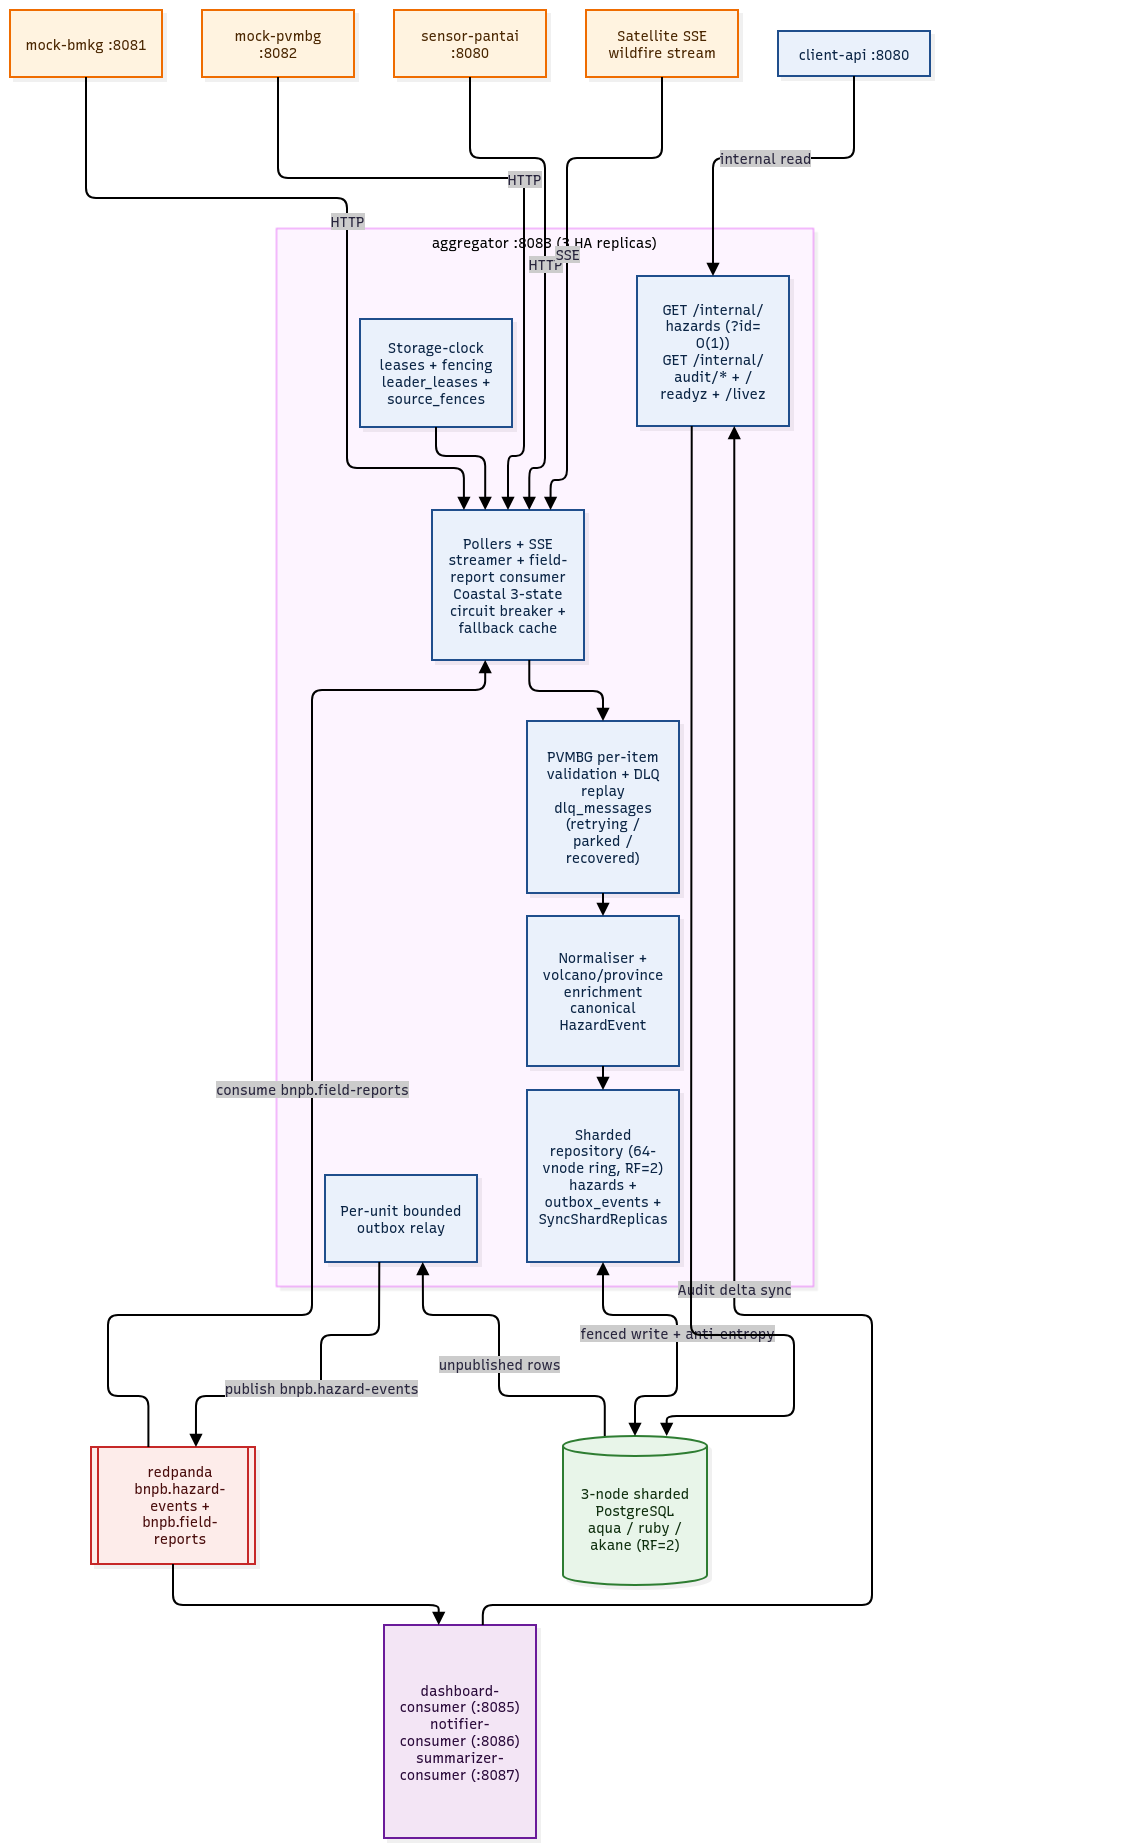
\includegraphics[width=\textwidth, height=16.5cm, keepaspectratio]{figures/aggregator.drawio.png}
        \caption{Alur ingesti multi-sumber, validasi DLQ, persistensi terpartisi ($RF=2$), dan \textit{outbox relay} pada \texttt{aggregator}.}
        \label{fig:alur_aggregator}
    \end{subfigure}\hfill
    \begin{subfigure}[t]{0.36\textwidth}
        \centering
        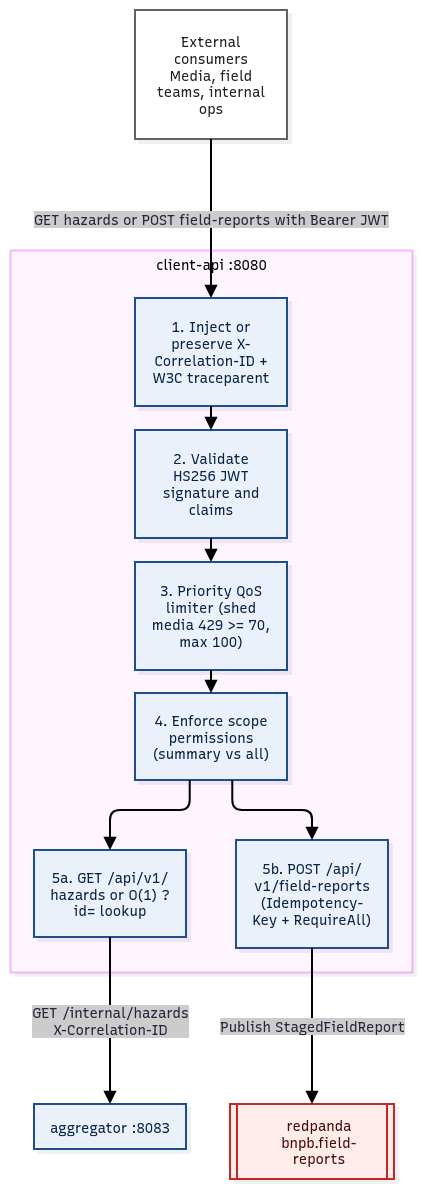
\includegraphics[width=\textwidth, height=16.5cm, keepaspectratio]{figures/client-api.drawio.png}
        \caption{Alur validasi JWT, \textit{Priority QoS}, jalur baca, dan \textit{staging} laporan lapangan pada \texttt{client-api}.}
        \label{fig:alur_client_api}
    \end{subfigure}
    \caption{Alur Permintaan, Ingesti Multi-Sumber, Persistensi Terpartisi, dan Distribusi Event Milestone~2.}
    \label{fig:alur_data_event}
\end{figure}

\clearpage
\section{Teknologi Terpilih dan Alasan Pemilihan}
\label{sec:teknologi_terpilih}

Tabel~\ref{tab:pemilihan_teknologi} merangkum tumpukan teknologi yang dipilih pada Milestone 2 beserta alasan pemilihan dan kesesuaiannya terhadap tuntutan sistem terdistribusi multi-node.

\begin{footnotesize}
\begin{spacing}{1.05}
\begin{xltabular}{\textwidth}{p{3.2cm} p{4.3cm} X}
\caption{Rangkuman Pemilihan Teknologi} \label{tab:pemilihan_teknologi} \\
\toprule
\textbf{Kategori} & \textbf{Teknologi} & \textbf{Alasan Pemilihan} \\
\midrule
\endfirsthead

\multicolumn{3}{l}{\textit{\footnotesize Lanjutan Tabel \ref{tab:pemilihan_teknologi}}} \\
\toprule
\textbf{Kategori} & \textbf{Teknologi} & \textbf{Alasan Pemilihan} \\
\midrule
\endhead

\bottomrule
\endfoot

Back-End & Go 1.22 (\texttt{pgx/v5}, \texttt{kafka-go}, \texttt{jwt/v5}) & Mendukung konkurensi ringan via \textit{goroutine} dan \textit{channel}, menghasilkan biner statis berukuran kecil untuk batas memori ketat, serta menyeragamkan seluruh layanan dalam delapan modul independen. \\
\addlinespace
Database Kanonis & PostgreSQL 16 (JSONB \& indeks GIN) & Menyediakan transaksi ACID untuk pola \textit{Transactional Outbox}, jam penyimpanan \texttt{clock\_timestamp()} untuk \textit{leader leasing} tahan \textit{clock skew}, serta fleksibilitas skema dinamis tanpa migrasi DDL. \\
\addlinespace
Orkestrasi \& Infrastruktur & Kubernetes (k3s \texttt{v1.37.2}), Traefik, Docker \& Docker Compose & Mendukung penjadwalan multi-node berkernel terpisah, penegakan isolasi via \texttt{NetworkPolicy}, tata kelola \texttt{LimitRange}, penskalaan otomatis HPA, serta simulasi lokal via Compose. \\
\addlinespace
Komunikasi Antarservice & HTTP/1.1 REST (JSON) \& \textit{Server-Sent Events} (SSE) & Menjamin antarmuka sinkron yang jelas, mendukung propagasi \texttt{X-Correlation-ID} dan \texttt{traceparent}, serta memungkinkan aliran dorong kontinu untuk data titik api satelit. \\
\addlinespace
Message Broker & Redpanda \texttt{v24.1.1} (API Kafka) & Kompatibel dengan protokol Kafka tanpa ketergantungan JVM maupun Zookeeper, mendukung \textit{durable staging} laporan lapangan serta distribusi \textit{fan-out} independen dengan pemulihan \textit{offset}. \\
\addlinespace
Autentikasi \& Otorisasi & JWT HS256, \textit{Refresh Token}, \& Bearer Token & Memungkinkan validasi klaim \textit{scope} secara lokal di gerbang API tanpa kueri silang antarnode, rotasi token berkala, serta proteksi rute audit dan hulu. \\
\addlinespace
Observabilitas & Prometheus \texttt{v2.54.1}, Grafana Tempo \texttt{v2.6.0} (OTLP), \& Grafana \texttt{v11.2.2} & Mengumpulkan metrik kinerja per replika pod, melacak latensi lintas layanan melalui \textit{distributed tracing} W3C, dan memantau kesehatan kluster secara waktu nyata. \\
\addlinespace
Inferensi AI Lokal & \texttt{llama-server} (\texttt{qwen3.5:9b}) \& \textit{Extractive Fallback} & Memungkinkan perangkuman situasional bencana berbasis LLM di jaringan LAN tanpa biaya per-token maupun ketergantungan SaaS eksternal, disertai \textit{fallback} deterministik saat beban tinggi. \\
\addlinespace
Dokumentasi Kontrak API & OpenAPI 3.0 \& JSON Schema & Menetapkan kontrak beku antarlayanan dan skema kanonis \texttt{HazardEvent} agar integrasi antarmodul serta audit tetap konsisten. \\
\addlinespace
Pengujian \& Automasi & \texttt{k6}, \texttt{curl}, \texttt{jq}, Python 3, \texttt{tester-agent}, Make, \& GitHub & Memfasilitasi uji beban hingga 10.000 VU, simulasi \textit{chaos engineering} multi-node, verifikasi parity checksum SHA-256, serta otomatisasi alur kerja melalui \texttt{Makefile}. \\
\end{xltabular}
\end{spacing}
\end{footnotesize}

\clearpage
\section{Diagram Deployment dan Deklarasi Topologi}

\begin{figure}[H]
    \centering
    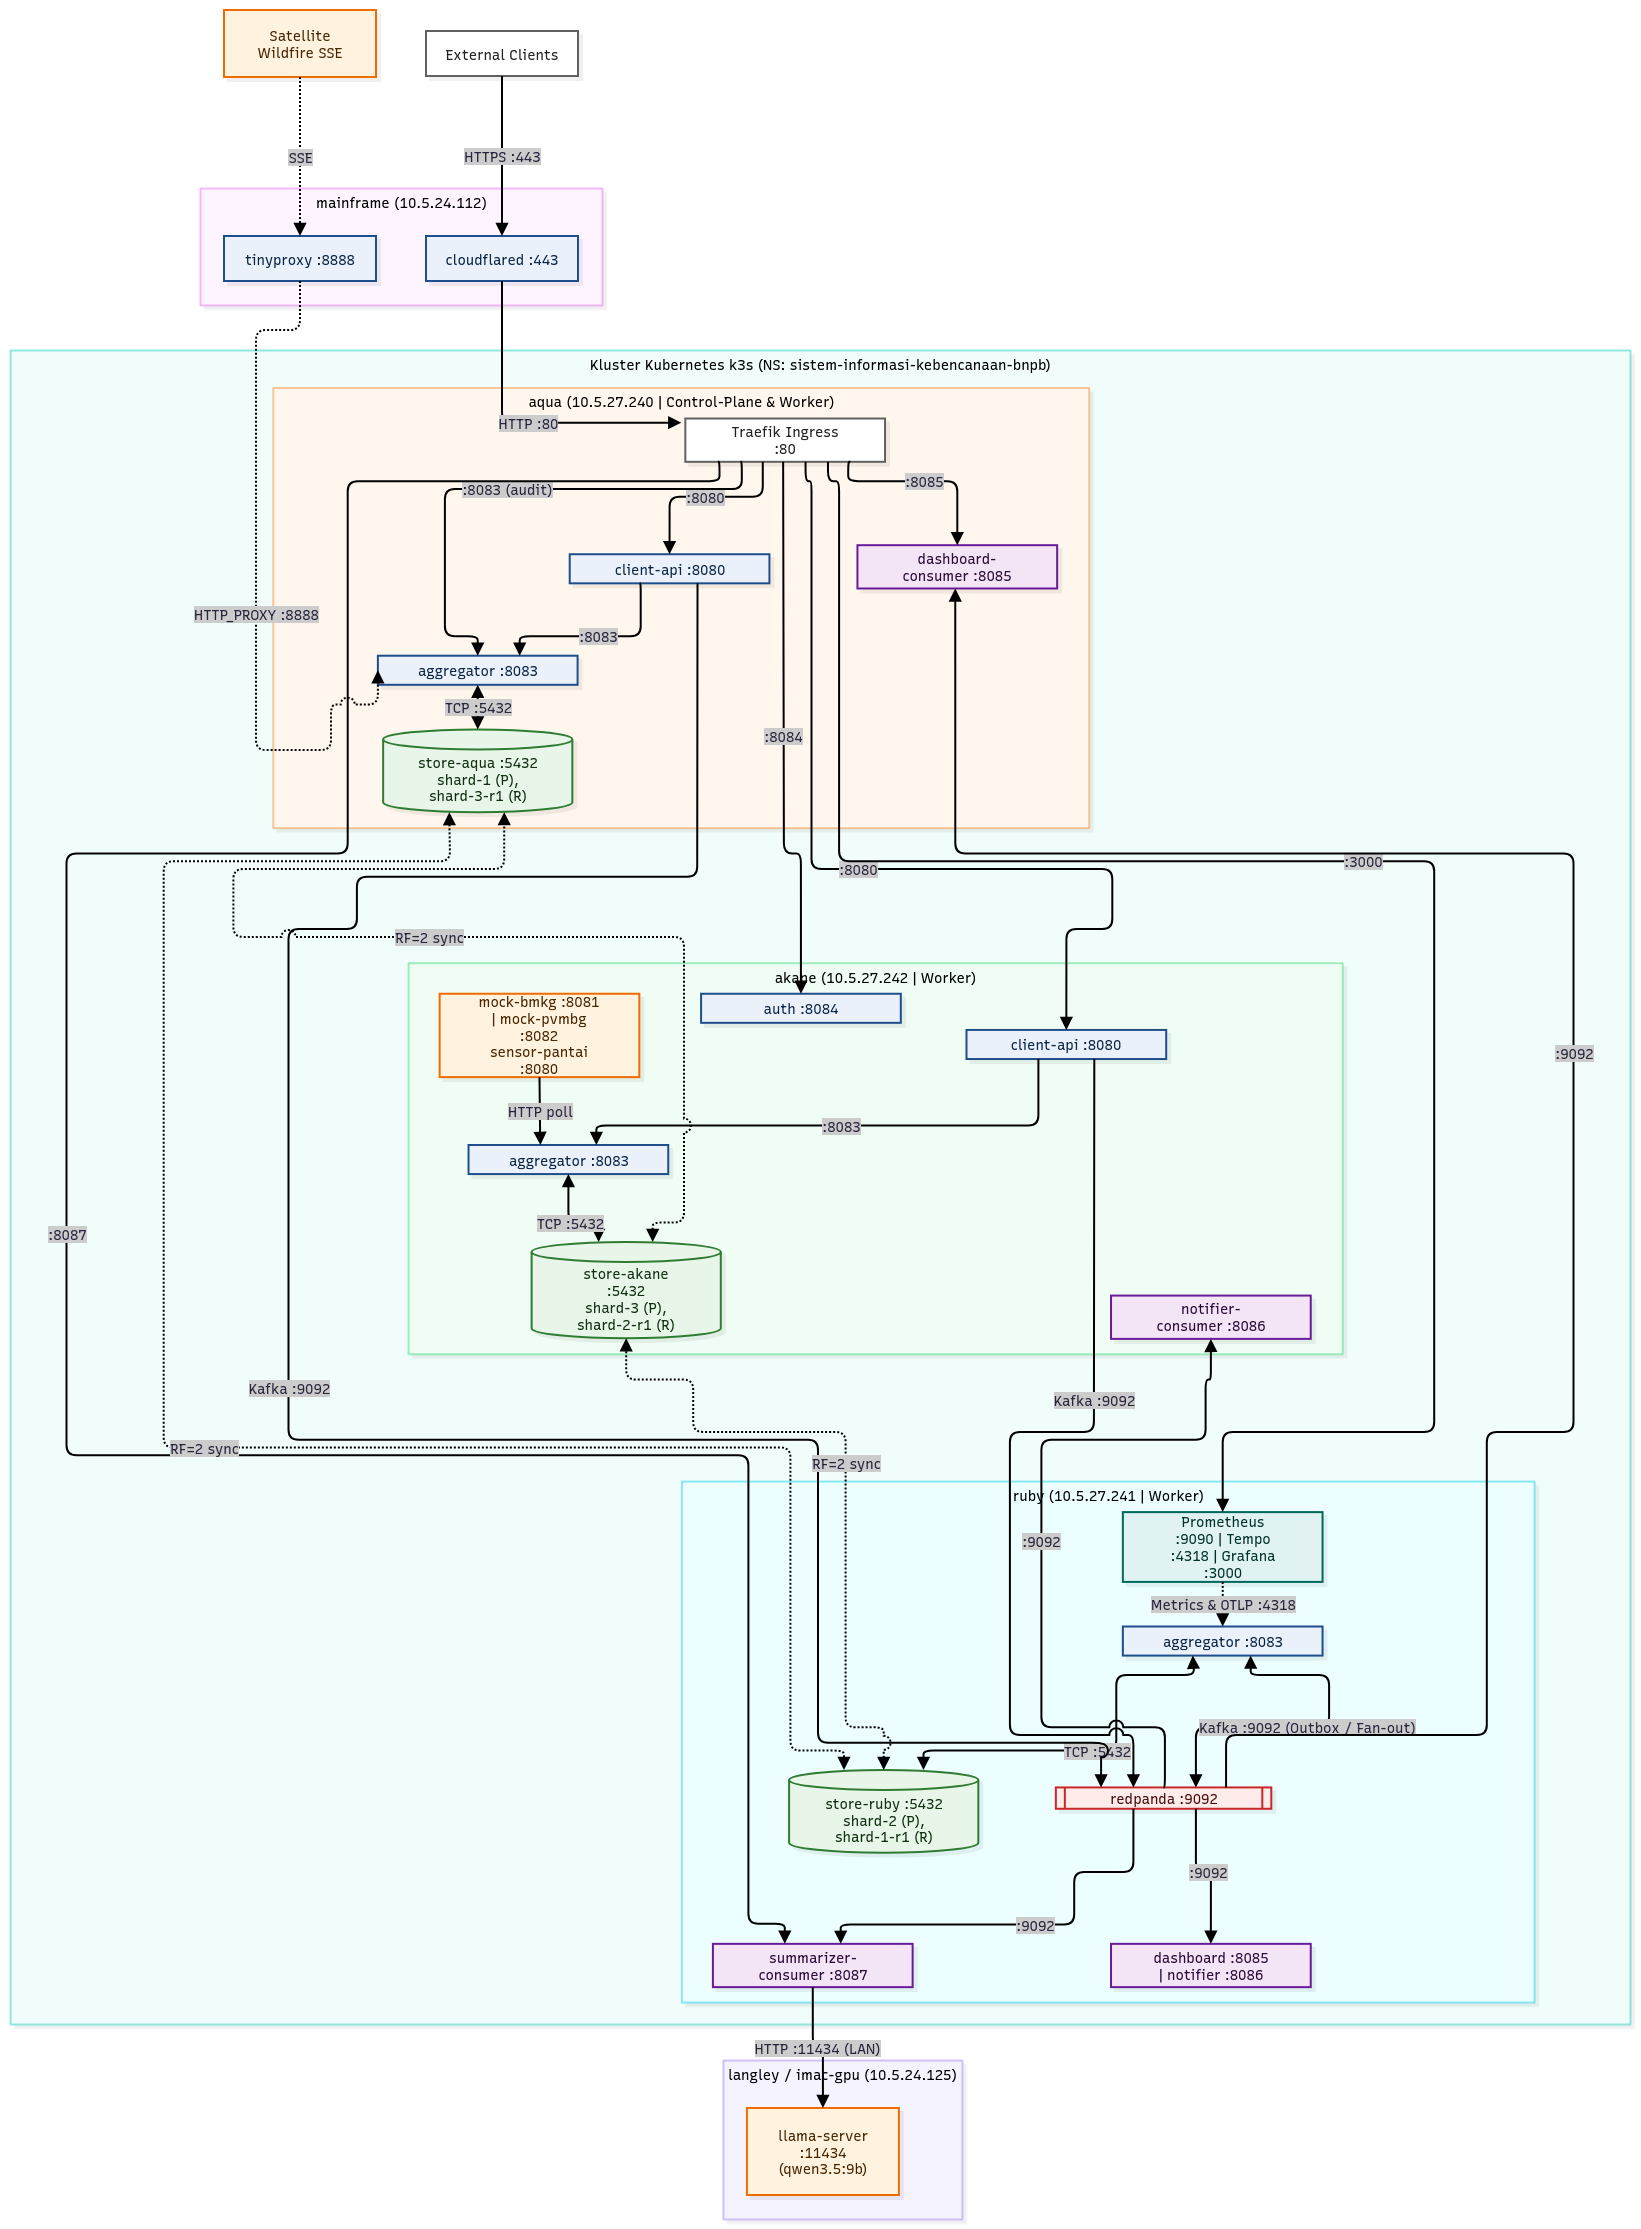
\includegraphics[width=0.92\textwidth, height=0.80\textheight, keepaspectratio]{figures/topologi.drawio.png}
    \caption{Diagram \textit{Deployment} dan Jalur Data Antar-Node Kluster Kubernetes 3-Node (\texttt{aqua}, \texttt{ruby}, \texttt{akane}) beserta Host Pendukung (\texttt{mainframe}, \texttt{langley}).}
    \label{fig:deployment_topologi}
\end{figure}

\noindent Kluster Kubernetes dijalankan di atas tiga mesin virtual QEMU/KVM terisolasi berkernel Linux terpisah yang di-\textit{host} pada tiga mesin fisik (\textit{bare-metal}) Lab Sister berbeda dalam subnet \texttt{10.5.24.0/22} dengan sistem operasi Debian~13, orkestrator \textbf{k3s \texttt{v1.37.2+k3s1}}, serta \textit{container runtime} \texttt{containerd://2.3.7-k3s1} (Gambar~\ref{fig:deployment_topologi} dan Tabel~\ref{tab:deklarasi_lingkungan}).

{\footnotesize
\setlength{\tabcolsep}{4.5pt}
\renewcommand{\arraystretch}{1.2}
\begin{spacing}{1.05}
\begin{xltabular}{\textwidth}{>{\raggedright\arraybackslash}p{1.3cm} >{\raggedright\arraybackslash}p{2.2cm} >{\raggedright\arraybackslash}p{3.4cm} >{\raggedright\arraybackslash}X >{\raggedright\arraybackslash}p{3.2cm}}
\caption{Lingkungan dan Spesifikasi Node Kluster Kubernetes} \label{tab:deklarasi_lingkungan} \\
\toprule
\textbf{Node} & \textbf{Host Fisik (\texttt{10.5.24.x})} & \textbf{Hardware Host \& Service} & \textbf{Peran Guest \& OS/Kernel} & \textbf{Resource Guest \& IP} \\
\midrule
\endfirsthead

\multicolumn{5}{l}{\textit{\footnotesize Lanjutan Tabel \ref{tab:deklarasi_lingkungan}}} \\
\toprule
\textbf{Node} & \textbf{Host Fisik (\texttt{10.5.24.x})} & \textbf{Hardware Host \& Service} & \textbf{Peran Guest \& OS/Kernel} & \textbf{Resource Guest \& IP} \\
\midrule
\endhead

\bottomrule
\endfoot

\textbf{\texttt{aqua}} &
\texttt{nexus} \newline (\texttt{10.5.24.111}) &
Intel Core i5-10500T \newline (6C/12T), 8~GB RAM, \newline 1~TB HDD \newline \texttt{aat-aqua.service} &
\textit{Control-plane} \& \textit{worker} \newline Debian~13 \newline \texttt{6.12.117+deb13-cloud-amd64} &
2~vCPU, 3,5~GB RAM \newline 40~GB disk \newline IP: \texttt{10.5.27.240} \\
\midrule
\textbf{\texttt{ruby}} &
\texttt{runner-1} \newline (\texttt{10.5.24.114}) &
Intel Core i5-10500T \newline (6C/12T), 8~GB RAM, \newline 1~TB HDD \newline \texttt{aat-ruby.service} &
\textit{Worker} non-\textit{control-plane} \newline Debian~13 \newline \texttt{6.12.117+deb13-cloud-amd64} &
2~vCPU, 3,5~GB RAM \newline 40~GB disk \newline IP: \texttt{10.5.27.241} \\
\midrule
\textbf{\texttt{akane}} &
\texttt{runner-2} \newline (\texttt{10.5.24.115}) &
Intel Core i5-10500T \newline (6C/12T), 8~GB RAM, \newline 1~TB HDD \newline \texttt{aat-akane.service} &
\textit{Worker} kedua (\textit{sharding} 3-node) \newline Debian~13 \newline \texttt{6.12.115+deb13.1-cloud-amd64} &
2~vCPU, 3,5~GB RAM \newline (3,3~GiB \textit{usable}) \newline 40~GB disk \newline IP: \texttt{10.5.27.242} \\
\end{xltabular}
\end{spacing}
}

\noindent Infrastruktur pendukung eksternal yang terhubung ke kluster meliputi:
\begin{itemize}
    \item \textbf{\texttt{mainframe} (\texttt{10.5.24.112}):} Intel Core i5-10500T, 8~GB RAM, Debian~13; berperan sebagai \textit{SSH bastion} Cloudflare Zero Trust (\texttt{ssh.sister.works}), \textit{gateway} Tunnel menuju \texttt{k8s-aat.darsu.dev} (Kubernetes API) serta \texttt{aat.darsu.dev} / \texttt{audit-aat.darsu.dev} (Traefik Ingress aplikasi), dan \textit{egress proxy} LAN (\texttt{tinyproxy :8888}) untuk lalu lintas HTTPS keluar bagi aliran SSE satelit pada \texttt{aggregator}.
    \item \textbf{\texttt{langley} / \texttt{imac-gpu} (\texttt{10.5.24.125}):} Intel Core iMac dengan AMD Radeon Pro 5500~XT (8~GiB VRAM, macOS); menjalankan \texttt{llama-server} (\texttt{works.sister.llama-server}, Vulkan/\allowbreak MoltenVK) untuk menyajikan model \texttt{Qwen3.5-9B-\allowbreak Q4\_K\_M} (\texttt{qwen3.5:9b}) pada port \texttt{:11434} di LAN \texttt{10.5.24.0/22} bagi \texttt{summarizer-consumer} (serta eksternal melalui Cloudflare Access \texttt{ai.sister.works}).
    \item \textbf{Citra VM Dasar (\textit{Golden VM Images}):} Ketiga VM menyimpan \textit{snapshot} dasar \texttt{vm-<nama>-golden.qcow2} pada host fisiknya hanya untuk persiapan pra-uji dan tidak pernah dipulihkan selama jendela pemulihan mandiri (\textit{self-recovery}).
\end{itemize}

\vspace{1em}

\noindent Seluruh pod aplikasi berjalan dalam namespace \texttt{sistem-informasi-\allowbreak kebencanaan-bnpb} (CIDR pod \texttt{10.42.0.0/16}, CIDR service \texttt{10.43.0.0/16}) dengan tata kelola \texttt{LimitRange} (\texttt{table-b-resource-limits}: default CPU \texttt{100m}/\texttt{500m}, batas maks. \texttt{2000m}/\texttt{1Gi}), lima aturan \texttt{NetworkPolicy} serta \texttt{tester-agent}. Lingkungan Docker Compose dipakai khusus untuk pengembangan lokal dan tidak menggantikan pengujian kegagalan multi-node berkernel terpisah. Alokasi per kelas komponen dirangkum pada Tabel~\ref{tab:deklarasi_workload}.

{\footnotesize
\renewcommand{\arraystretch}{1.18}
\begin{spacing}{1.05}
\begin{xltabular}{\textwidth}{>{\raggedright\arraybackslash}p{3.4cm} >{\raggedright\arraybackslash}X >{\raggedright\arraybackslash}p{2.3cm} >{\raggedright\arraybackslash}p{3.7cm}}
\caption{Konvensi dan Alokasi Sumber Daya Workload} \label{tab:deklarasi_workload} \\
\toprule
\textbf{Kelas Komponen} & \textbf{Role \& Layanan} & \textbf{Replika} & \textbf{Alokasi Memori \& CPU} \\
\midrule
\endfirsthead

\multicolumn{4}{l}{\textit{\footnotesize Lanjutan Tabel \ref{tab:deklarasi_workload}}} \\
\toprule
\textbf{Kelas Komponen} & \textbf{Role \& Layanan} & \textbf{Replika} & \textbf{Alokasi Memori \& CPU} \\
\midrule
\endhead

\bottomrule
\endfoot

Aggregator &
\texttt{role=aggregator}: \texttt{aggregator} &
\texttt{3} (HPA \texttt{3--5}) &
Mem \texttt{256Mi}/\texttt{512Mi}; CPU req \texttt{250m} \\
\midrule
Storage instance &
\texttt{role=store}: \texttt{store-aqua}, \texttt{store-ruby}, \texttt{store-akane} (PostgreSQL~16) &
\texttt{1}/node (\texttt{3} total) &
Mem \texttt{512Mi}/\texttt{1Gi} (\texttt{hostPath}) \\
\midrule
Broker / stream processor &
\texttt{role=broker}: \texttt{redpanda} (\texttt{v24.1.1}) \& \texttt{redpanda-topic-init} &
\texttt{1} &
Mem \texttt{512Mi}/\texttt{1Gi} (\texttt{hostPath}) \\
\midrule
Consumer / event processor &
\texttt{role=consumer}: \texttt{dashboard-consumer}, \texttt{notifier-consumer}, \texttt{summarizer-consumer} &
\texttt{2} / \texttt{2} / \texttt{1} &
Mem \texttt{128Mi}/\texttt{256Mi} \newline (\texttt{GOMEMLIMIT=200MiB}) \\
\midrule
Auth / Client API &
\texttt{role=api}: \texttt{auth}, \texttt{client-api} &
\texttt{1} / \texttt{2} (HPA \texttt{2--6}) &
Mem \texttt{128Mi}/\texttt{256Mi}; \texttt{client-api} CPU req \texttt{100m} \\
\midrule
BMKG / PVMBG mock &
\texttt{role=mock}: \texttt{mock-bmkg}, \texttt{mock-pvmbg} &
\texttt{1} / \texttt{1} &
Mem \texttt{64Mi}/\texttt{128Mi} \\
\midrule
Other components &
\texttt{role=sensor}: \texttt{sensor-pantai} \newline \texttt{role=other}: \texttt{prometheus}, \texttt{tempo}, \texttt{grafana} &
\texttt{1} masing-masing &
Mem \texttt{128Mi}/\texttt{256Mi} \\
\end{xltabular}
\end{spacing}
}

StatefulSet penyimpanan dan broker \texttt{redpanda} diikat tetap ke node tertentu menggunakan \texttt{nodeSelector}. Layanan \texttt{aggregator} disebar merata lintas tiga node melalui \texttt{topologySpreadConstraints} dan \texttt{podAntiAffinity}, layanan \textit{stateless} multi-replika memakai \texttt{podAntiAffinity} preferensial, sedangkan layanan replika tunggal pada Tabel~\ref{tab:deklarasi_topologi} mencerminkan penempatan \textit{baseline} yang teramati pada kluster.

{\footnotesize
\renewcommand{\arraystretch}{1.2}
\begin{spacing}{1.05}
\begin{xltabular}{\textwidth}{>{\raggedright\arraybackslash}p{2.8cm} >{\raggedright\arraybackslash}X >{\raggedright\arraybackslash}p{5.6cm}}
\caption{Pemetaan Komponen serta Jalur Data dan Port per Node/Host} \label{tab:deklarasi_topologi} \\
\toprule
\textbf{Node / Host} & \textbf{Komponen / Service yang Dijalankan} & \textbf{Jalur Data \& Port} \\
\midrule
\endfirsthead

\multicolumn{3}{l}{\textit{\footnotesize Lanjutan Tabel \ref{tab:deklarasi_topologi}}} \\
\toprule
\textbf{Node / Host} & \textbf{Komponen / Service yang Dijalankan} & \textbf{Jalur Data \& Port} \\
\midrule
\endhead

\bottomrule
\endfoot

\textbf{\texttt{aqua}} \newline \texttt{10.5.27.240} \newline \textit{Control-plane \& Worker} &
\textbf{Pinned:} \texttt{store-aqua} (\texttt{shard-1} primer, \texttt{shard-3-r1} replika, \texttt{hostPath}) \newline
\textbf{Aplikasi:} \texttt{aggregator} (1/3), \texttt{client-api} (1/2), \texttt{dashboard-consumer} (1/2) \newline
\textbf{Sistem:} k3s \textit{control-plane}, Traefik Ingress, \texttt{tester-agent} (\textit{DaemonSet}) &
HTTP \texttt{:80} (Traefik Ingress) \newline
TCP \texttt{:6443} (Kubernetes API) \newline
HTTP \texttt{:8080} (\texttt{client-api}), \texttt{:8083} (\texttt{aggregator}) \newline
HTTP \texttt{:8085} (\texttt{dashboard-consumer}) \newline
TCP \texttt{:5432} (PostgreSQL, terisolasi) \\
\midrule
\textbf{\texttt{ruby}} \newline \texttt{10.5.27.241} \newline \textit{Worker} \newline (\textit{Target Chaos}) &
\textbf{Pinned:} \texttt{store-ruby} (\texttt{shard-2} primer, \texttt{shard-1-r1} replika, \texttt{hostPath}), \texttt{redpanda} (\texttt{v24.1.1}, 3~partisi/topik, \texttt{hostPath}) \newline
\textbf{Aplikasi:} \texttt{aggregator} (1/3), \texttt{dashboard-consumer} (1/2), \texttt{notifier-consumer} (1/2), \texttt{summarizer-consumer} \newline
\textbf{Obs/Sistem:} \texttt{prometheus}, \texttt{tempo}, \texttt{grafana}, \texttt{tester-agent} &
TCP \texttt{:5432} (PostgreSQL) \newline
TCP \texttt{:9092} (Kafka), \texttt{:9644} (Redpanda Admin) \newline
HTTP \texttt{:8083} (\texttt{aggregator}) \newline
HTTP \texttt{:8085} (\texttt{dashboard}), \texttt{:8086} (\texttt{notifier}), \texttt{:8087} (\texttt{summarizer}) \newline
Obs: \texttt{:9090} (Prom), \texttt{:3200}/\texttt{:4318} (Tempo), \texttt{:3000} (Grafana) \\
\midrule
\textbf{\texttt{akane}} \newline \texttt{10.5.27.242} \newline \textit{Worker} \newline (\textit{Target Chaos}) &
\textbf{Pinned:} \texttt{store-akane} (\texttt{shard-3} primer, \texttt{shard-2-r1} replika, \texttt{hostPath}) \newline
\textbf{Aplikasi:} \texttt{aggregator} (1/3), \texttt{client-api} (1/2), \texttt{auth}, \texttt{notifier-consumer} (1/2) \newline
\textbf{Hulu/Sistem:} \texttt{mock-bmkg}, \texttt{mock-pvmbg}, \texttt{sensor-pantai}, \texttt{tester-agent} &
TCP \texttt{:5432} (PostgreSQL) \newline
HTTP \texttt{:8080} (\texttt{client-api}), \texttt{:8083} (\texttt{aggregator}) \newline
HTTP \texttt{:8084} (\texttt{auth}), \texttt{:8086} (\texttt{notifier-consumer}) \newline
HTTP \texttt{:8081} (BMKG), \texttt{:8082} (PVMBG), \texttt{:8080} (\texttt{sensor-pantai}) \\
\midrule
\textbf{\texttt{mainframe}} \newline \texttt{10.5.24.112} \newline \textit{Gateway \& Proxy} &
\textbf{Layanan:} Cloudflare Tunnel (\texttt{cloudflared}), \texttt{tinyproxy} (\textit{WARP egress proxy} SSE satelit) \newline
\textbf{Pengujian:} Host \textit{load generator} eksternal (\texttt{k6} / Go 10.000~VU) &
HTTPS \texttt{:443} (Tunnel): \texttt{aat.darsu.dev}, \texttt{audit-aat.darsu.dev}, \texttt{k8s-aat.darsu.dev} \newline
HTTP/HTTPS \texttt{:8888} (\texttt{tinyproxy} \textit{egress} LAN) \\
\midrule
\textbf{\texttt{langley} / \texttt{imac-gpu}} \newline \texttt{10.5.24.125} \newline \textit{AI Inference Host} &
\textbf{Layanan:} \texttt{llama-server} (Vulkan/\allowbreak MoltenVK) menyajikan model \texttt{Qwen3.5-9B-\allowbreak Q4\_K\_M} (\texttt{qwen3.5:9b}) untuk \texttt{summarizer-consumer} &
HTTP REST \texttt{:11434} (LAN \texttt{10.5.24.0/22}) \newline
HTTPS (Cloudflare Access: \texttt{ai.sister.works}) \\
\end{xltabular}
\end{spacing}
}
